\documentclass[12pt]{article}

\usepackage[utf8]{inputenc}
\usepackage[english]{babel}
\usepackage{amssymb}
\usepackage{amsfonts}
\usepackage{amsmath}
\usepackage{graphicx}
\usepackage[margin=1in]{geometry}
\usepackage[hidelinks]{hyperref}
\usepackage{float}
\usepackage[danish]{varioref}
\usepackage{multirow}
\usepackage{hhline}
\usepackage{inconsolata}
\usepackage{etoolbox}
\usepackage[usenames,dvipsnames]{xcolor}
\usepackage{tikz}
\usetikzlibrary{positioning,shapes, shadows, arrows}
\usepackage{listings}

%%%%%%%%%%%%%%%%%%%%%%%%%
%   subsubsubsection    %

\usepackage{titlesec}
\titleclass{\subsubsubsection}{straight}[\subsection]

\newcounter{subsubsubsection}[subsubsection]
\renewcommand\thesubsubsubsection{\thesubsubsection.\arabic{subsubsubsection}}

\titleformat{\subsubsubsection}
  {\normalfont\normalsize\bfseries}{\thesubsubsubsection}{1em}{}
\titlespacing*{\subsubsubsection}
{0pt}{3.25ex plus 1ex minus .2ex}{1.5ex plus .2ex}

\makeatletter
\def\toclevel@subsubsubsection{4}
\def\l@subsubsubsection{\@dottedtocline{4}{7em}{4em}}
\makeatother

\setcounter{secnumdepth}{4}
\setcounter{tocdepth}{4}

%                       %
%%%%%%%%%%%%%%%%%%%%%%%%%

%%%%%%%%%%%%%%%%%%%%%%%%%
%          Tikz         %

\tikzset{
  treenode/.style = {align=center, inner sep=0pt, text centered,
    font=\sffamily},
  arn_n/.style = {treenode, circle, black, font=\sffamily\bfseries, draw=white, fill=white, text width=1.5em}
}

%                       %
%%%%%%%%%%%%%%%%%%%%%%%%%    

\setlength\parindent{0pt}
\usepackage[parfill]{parskip}

\definecolor{dark-blue}{HTML}{000080}
\definecolor{dark-green}{HTML}{008000}
\definecolor{pale-purple}{HTML}{94558D}
\definecolor{dark-purple}{HTML}{0000AA}
\definecolor{regular-purple}{HTML}{660099}
\definecolor{magenta}{HTML}{B200B2}
\definecolor{light-gray}{HTML}{FAFAFA}
\definecolor{dark-gray}{HTML}{2D2D2D}
\definecolor{comment}{HTML}{808080}
\definecolor{digit}{HTML}{0000FF}

\newcommand*{\FormatDigit}[1]{\textcolor{digit}{#1}}

\lstset{
	language=Ruby,
	prebreak=\raisebox{0ex}[0ex][0ex]{\ensuremath{\color{red}\space\hookleftarrow}},
	basicstyle=\footnotesize\ttfamily,
	%
	literate=%
    	{0}{{\FormatDigit{0}}}{1}%
        {1}{{\FormatDigit{1}}}{1}%
        {2}{{\FormatDigit{2}}}{1}%
        {3}{{\FormatDigit{3}}}{1}%
        {4}{{\FormatDigit{4}}}{1}%
        {5}{{\FormatDigit{5}}}{1}%
        {6}{{\FormatDigit{6}}}{1}%
        {7}{{\FormatDigit{7}}}{1}%
        {8}{{\FormatDigit{8}}}{1}%
        {9}{{\FormatDigit{9}}}{1}%
        {.0}{{\FormatDigit{.0}}}{2}% Following is to ensure that only periods
        {.1}{{\FormatDigit{.1}}}{2}% followed by a digit are changed.
        {.2}{{\FormatDigit{.2}}}{2}%
        {.3}{{\FormatDigit{.3}}}{2}%
        {.4}{{\FormatDigit{.4}}}{2}%
        {.5}{{\FormatDigit{.5}}}{2}%
        {.6}{{\FormatDigit{.6}}}{2}%
        {.7}{{\FormatDigit{.7}}}{2}%
        {.8}{{\FormatDigit{.8}}}{2}%
        {.9}{{\FormatDigit{.9}}}{2}%
        %{,}{{\FormatDigit{,}}{1}% depends if you want the "," in color
        {\ }{{ }}{1}% handle the space
		{æ}{{\ae}}1
        {ø}{{\o}}1
        {å}{{\aa}}1
        {Æ}{{\AE}}1	
        {Ø}{{\O}}1
        {Å}{{\AA}}1
        {~}{{$\scriptstyle{\sim}$}}1, % handle tilde ~
	%
	%emph={@param,@return},
	otherkeywords={},
	keywords=[2]{self},
	keywords=[3]{__init__},
	keywords=[4]{object},
	keywords=[5]{encoding, flags},
	keywords=[6]{map},
	%
	keywordstyle=\bfseries\color{dark-blue},
	keywordstyle={[2]\color{pale-purple}},
	keywordstyle={[3]\color{magenta}},
	keywordstyle={[4]\color{dark-blue}},
	keywordstyle={[5]\color{regular-purple}},
	keywordstyle={[6]\color{dark-purple}},
	keywordstyle={[7]\bfseries\color{black}},
    commentstyle=\itshape\color{comment},
    identifierstyle=\color{black},
	stringstyle=\bfseries\color{dark-green},
	%emphstyle=\bfseries,
	%
	numbers=left, % where to put the line-numbers
	numberstyle=\ttfamily\color{dark-gray},
	numbersep=5pt, % how far the line-numbers are from the code
	stepnumber=1,
	showstringspaces=false,
	backgroundcolor=\color{light-gray},
	tabsize=4,
	captionpos=b, % sets the caption-position to bottom
	breaklines=true % sets automatic line breaking
}

\linespread{1.3}

\begin{document}

\begin{titlepage}
    \vspace*{\fill}
    \begin{center}
      {\Huge Midtvejsrapport Bachelorproject}\\[0.7cm]
      {\Large Regular Expression Matching In Genomic Data}\\[0.4cm]
      {\large Rasmus Haarslev - nkh877}\\
      {\large Troels Thomsen - qvw203}\\[0.4cm]
      {Supervisors: Rasmus Fonseca}\\
      {\small 23. Februar 2015}\\[0.3cm] 
      {\small Department of Computer Science}\\
      {\small University of Copenhagen}
    \end{center}
    \vspace*{\fill}
\end{titlepage}	

\clearpage
\pagenumbering{gobble}
\thispagestyle{empty}

\newpage

\tableofcontents
\newpage

\pagenumbering{arabic}

\section{Problem definition}

We wish to determine the possibility of converting sequence analysis patterns used for scan-for-matches\cite{scan-for-matches}, into regular expressions\cite{crash-course-regex} and test their efficiency against the KMC\cite{kmc-website} engine.

Specifically we wish to solve the following problems:

\begin{itemize}
	\item Is it possible to programatically convert patterns used by the scan-for-matches program into regular expressions for the KMC engine? If not all patterns used by scan-for-matches then which ones?
	\item Is it possible to achieve speeds matching or exceeding scan-for-matches with the generated regular expressions and the KMC engine?
	\item Can we find weak extensions to regular expressions, which would enable us to support more or all scan-for-matches patterns?
\end{itemize}

\newpage

\section{Introduction}

Scan for matches is a program developed by Ross Overbeek, David Joerg and Morgan Price, which is able to locate complex DNA patterns.\cite{scan-for-matches} These patterns are written in their own language, which from now on will be referred to as patscan patterns, while the program itself will be referred to as scan-for-matches.

The patscan language can be broken down into a few simple components or tokens, which we will refer to as sub-patterns. We have divided the sub-patterns into the following classes: \textit{sequences} (\texttt{AGTCT}), \textit{sequences with mismatches, insertions and deletions} (\texttt{AGTCT[1,0,0]}) which we will refer to as combinations, \textit{ranges} (\texttt{2...4}), \textit{variable assignments} (\texttt{p1=AGTCT}) and finally \textit{variable usages} (\texttt{p1}). The complete grammar we use for our translation can be found in section \ref{Patscan grammar}.

The most notable of the patscan format's features, is the possibility to search for mismatches, insertions and deletions in a given sequence or stored sequence. The sequence \texttt{AGTCT} can be extended to \texttt{AGTCT[1,1,1]} in order to match up to one mismatch, up to one insertion, up to one deletion or any combination thereof. \\
This means that a sequence of length $n$ with a single mismatch will yield $n^1+1$ possible matches. \texttt{AGTCT[1,0,0]} will for instance match any of the following, where \_ represents a mismatch.

\texttt{AGTCT, \_GTCT, A\_TCT, AG\_CT, AGT\_T, AGTC\_}

If we extrapolate into $m$ mismatches, $d$ deletions, and $i$ insertions, we quickly find ourselves with approximately  $n^{m^{d^{i}}}+1$ possible matches since all of our mismatches can be combined with all of our deletions, which in turn can be combined with all of our insertions. This is not something easily replicated with regular expressions, as we shall see in the following sections.

Another powerful feature of patscan is the ability to store a sub-pattern match in a named variable. If a match is found for the named variable in the beginning of a pattern for instance, this match can then be referenced later in the same pattern, by using the variable name. \\
An example of this could be the pattern \texttt{p1=2...4 10...20 \~{}p1}. This pattern will match the contents of \texttt{p1}, followed by any 10 to 20 characters, followed by the match stored in \texttt{p1}, but inverted as denoted by the \texttt{\~{}}.\\
This is similar to the back-referencing functionality for capturing groups, which many popular regular expression implementations support.%\cite{indsæt citation her.}

Combining this match combination notation with the ability to store sequences in variables and matching them further down the pattern, makes the patscan language very expressive compared to regular expressions. \\
A pattern as simple as \texttt{p1=8...16 10...50 ~p1[2,0,1]} describes a complex relationship, which cannot easily be discovered through conventional search methods.

We will try to translate patscan patterns into regular expressions, and run them on the KMC engine. We hope to achieve similar speeds to those of scan-for-matches, while also achieving the same search results.

\newpage

\section{What is regular expressions}

\newpage

\section{The KMC project}

\newpage

\section{PatScan as regular expressions}

\newpage

\section{Translation of scan-for-matches patterns into regular expressions}

\subsection{Grammar}
\label{Patscan grammar}

We have defined the following grammar for the patscan tokens / sub-patterns: \\

\begin{tabular}{ p{5cm} | l | l }
	\textbf{Token type} & \textbf{Regular expression} & \textbf{Example} \\
    \hline
    Sequence & 
  	{\begin{lstlisting}[numbers=none, backgroundcolor=\color{white}]
^[A-Z]+$ 
	\end{lstlisting}} & 
    {\begin{lstlisting}[numbers=none, backgroundcolor=\color{white}]
AGTCT
	\end{lstlisting}} \\
    \hline
    Sequence with mismatches, insertions and deletions & 
	{\begin{lstlisting}[numbers=none, backgroundcolor=\color{white}]
^[A-Z]+\[[0-9]+,[0-9]+,[0-9]+\]$ 
	\end{lstlisting}} &
    {\begin{lstlisting}[numbers=none, backgroundcolor=\color{white}]
AGTCT[1,0,0]
	\end{lstlisting}} \\
    \hline
    Range & 
	{\begin{lstlisting}[numbers=none, backgroundcolor=\color{white}]
^[0-9]+\.{3}[0-9]+$
	\end{lstlisting}} & 
	{\begin{lstlisting}[numbers=none, backgroundcolor=\color{white}]
2...4
	\end{lstlisting}} \\
    \hline
    Variable assignment & 
    {\begin{lstlisting}[numbers=none, backgroundcolor=\color{white}]
^[^=]+=[^=]+$
	\end{lstlisting}} & 
    {\begin{lstlisting}[numbers=none, backgroundcolor=\color{white}]
p1=4...8
	\end{lstlisting}} \\
    \hline
    Variable usage &
	{\begin{lstlisting}[numbers=none, backgroundcolor=\color{white}]
^~?[\^{}=]+$ 
	\end{lstlisting}} &
    {\begin{lstlisting}[numbers=none, backgroundcolor=\color{white}]
~p1
	\end{lstlisting}} \\
\end{tabular}

\subsection{Mismatches, Insertions and Deletions}

Sub-patterns can have the following form, which allows for mismatches, insertions and deletions in the sub-pattern. 

\begin{equation}
	x_1 \ldots x_n[m, i, d] \ \ \{ x_1 \ldots x_n \in A \ | \ m, i, d \in \mathbb{N}_0 \}
\end{equation} 

This notation allows for 0 or the given number of mismatches, insertions or deletions, or all possible combinations in between. This means we for example can have $m$ mismatches and $i$ insertions, but not necessarily $d$ deletions.

Translating these sub-patterns is not a simple task. This kind of notation does not exist in regular expressions, hence the only way to represent them is by constructing every possible combination of the sequence, matching the patscan notation. To give an example, the pattern \texttt{AAG[1,0,0]} will translate into 

\hspace*{\fill}
\texttt{((AAG)|([\^{}A]AG)|(A[\^{}A]G)|(AA[\^{}G]))}
\hspace*{\fill}

Starting with mismatches only, writing a general algorithm to translate this example is fairly simple, but becomes increasingly difficult, as the sequence becomes longer, and the number of allowed mismatches increases.

We tried the following approaches to solving this problem, but ultimately decided on a divide and conquer algorithm. 

\subsubsection{Loops}

At the first glance this might seem like the trivial implementation. A single mismatch using loops can be done by simply choosing a different character for the mismatch in each iteration.
But for every new mismatch dimension, we would need to add another nested loop, which would make our code extremely inflexible and difficult to understand.

\subsubsection{Recursion}

Solving the problem with recursion one might take each character one at a time, and look at all the possibilities for that character.

This way we could construct a recursion tree containing all possible combinations, no matter how many mismatches are allowed.

For mismatches the recursion tree would add two new branches per iteration. The first iteration of \texttt{AGCTC[2,0,0]} would add the branches

\begin{eqnarray}
	Left\ branch &=& A\{GCTC[2,0,0]\} \\
	right\ branch &=&\ \hat{}A\{GCTC[1,0,0]\}
\end{eqnarray}

The left branch will continue recursively with \texttt{GCTC[2,0,0]}, and the right branch will do the same but with only one mismatch available, since we already chose $A$ as our first mismatch. Thus we must choose all possibilities from $N \in \{n, \hat{}n\}$ as a new branch, every time we take a recursion step.
On our leafs we will have a string with a unique combination of mismatches.

Adding deletions and insertions will increase the size of $N$, thus drastically increasing the recursion depth. The recursion does not stop until every combination is found. This means that if the sequence is large enough (This can happen already at a length of 20, if not earlier, depending on the number of mismatches, insertions, and deletions), the program will reach maximum recursion depth or run out of memory before completing.

\subsubsection{Divide and Conquer}

To solve the recursion depth problem, we thought of using a divide and conquer algorithm instead, which reduces the recursion depth to $logn$. This works by splitting the sequence in two halves per recursion, so at the deepest recursion level, we have a sequence of only a single character.

\begin{figure}[H]
\begin{tikzpicture}[->,>=stealth',level/.style={sibling distance = 5cm/#1,
  level distance = 1.5cm}] 
\node [arn_n] {abcd}
	child{ node [arn_n] {ab} 
		child{ node [arn_n] {a}}
		child{ node [arn_n] {b}}                            
	}
    child{ node [arn_n] {cd}
		child{ node [arn_n] {c}}
		child{ node [arn_n] {d}}
	}
; 
\end{tikzpicture}
	\centering
	\caption{Tree structure, showing the steps taken by the algorithm during the divide step.}
	\label{fig:tree_example}
\end{figure}

After dividing the sequence into characters, we have to conquer each sub-problem. On the lowest recursion level (where the sequence is a single character), the algorithm will return a list of all possibilities, which that character can be.

For character 'a' from figure \ref{fig:tree_example}, we have the following possibilities for mismatches and deletions

\begin{center}
	{a, \^{}a, \_}
\end{center}

as well as the following for insertions

\begin{center}
	\texttt{.\{1\}a, .\{2\}a, $\cdots$, .\{n\}a} \\
	\texttt{a.\{1\}, a.\{2\}, $\cdots$, a.\{n\}}
\end{center}


\subsection{Variable assignments}


\subsection{Variable usage}


\section{Application flow chart}

\subsection{Lexer}
\begin{figure}[H]
	\begin{center}
		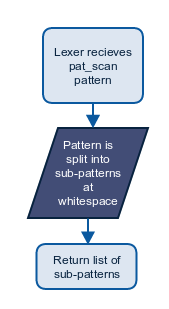
\includegraphics[scale=1]{lexer.png}
	\end{center}
	\caption{Flow chart of our lexer}
\end{figure}

Pat\_scan sub-patterns are separated by whitespace characters. Because of this, and because of the fact that the grammar is very simple, we can simply split the patcan pattern at each whitespace to get a list of sub-patterns, which we will refer to as tokens.

\subsection{Parser}
\begin{figure}[H]
	\begin{center}
		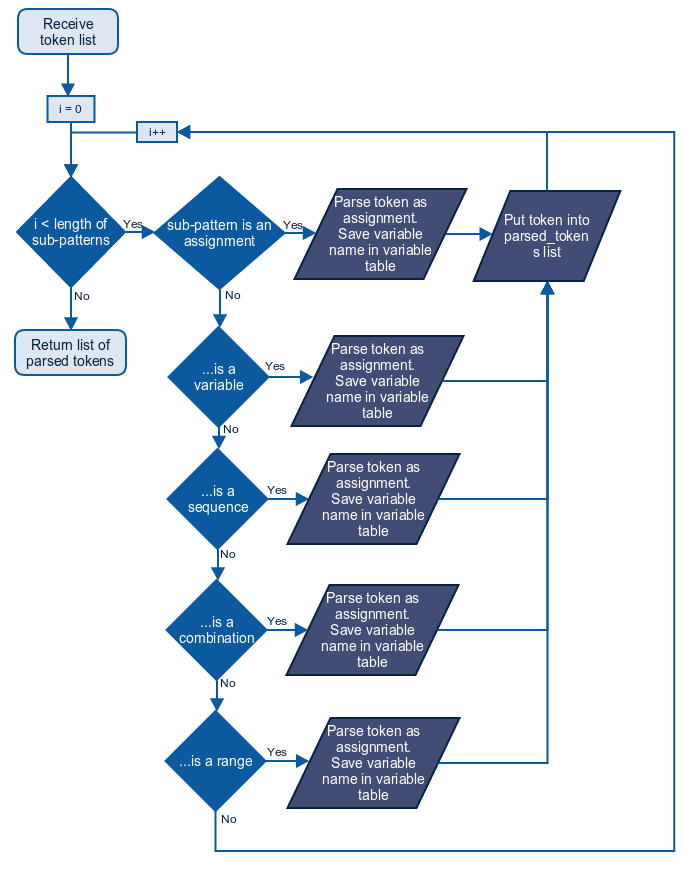
\includegraphics[scale=0.65]{parser.png}
	\end{center}	
	\caption{Flow chart of our parser}
\end{figure}

The parser takes each token from the lexer's token list, and checks them against our grammar. The tokens are then put into a Token objects, which takes a pattern type and a match object. \\
The pattern type enables the translator to recognize which type of sub-pattern the token belongs to. The match object is the regular expression object returned by our grammar. This match object contains information about the specific parts of our tokens, such as the number of mismatches belonging to a sequence such as \texttt{AGTCA[2,0,0]}.

\begin{figure}[H]
	\begin{lstlisting}
 	# Discover sequence with mismatch, insertion, deletion permutations
    #
    # @param [String] token_string
    # @return [MatchData]
    def get_combination(token_string)
        return /^(?<sequence>\w+)\[(?<mismatches>\d+),(?<insertions>\d+),(?<deletions>\d+)\]$/.match token_string
    end
	\end{lstlisting}
	\caption{Grammar for matching sequences with the amount of combinations.}
	\label{fig:gamme_c}
\end{figure}

\newpage

\section{Regular expression performance}

\subsection{Ruby}

\subsection{KMC}

\subsection{Google's engine}

\newpage

\bibliographystyle{plain}
%\nocite{*}
\bibliography{litterature}

\end{document}
